% Copyright 2004 by Till Tantau <tantau@users.sourceforge.net>.
%
% In principle, this file can be redistributed and/or modified under
% the terms of the GNU Public License, version 2.
%
% However, this file is supposed to be a template to be modified
% for your own needs. For this reason, if you use this file as a
% template and not specifically distribute it as part of a another
% package/program, I grant the extra permission to freely copy and
% modify this file as you see fit and even to delete this copyright
% notice. 

% \UseRawInputEncoding
\documentclass{beamer}

% There are many different themes available for Beamer. A comprehensive
% list with examples is given here:
% http://deic.uab.es/~iblanes/beamer_gallery/index_by_theme.html
% You can uncomment the themes below if you would like to use a different
% one:
%\usetheme{AnnArbor}
%\usetheme{Antibes}
%\usetheme{Bergen}
%\usetheme{Berkeley}
%\usetheme{Berlin}
%\usetheme{Boadilla}
%\usetheme{boxes}
%\usetheme{CambridgeUS}
%\usetheme{Copenhagen}
%\usetheme{Darmstadt}
%\usetheme{default}
%\usetheme{Frankfurt}
%\usetheme{Goettingen}
%\usetheme{Hannover}
%\usetheme{Ilmenau}
%\usetheme{JuanLesPins}
%\usetheme{Luebeck}
\usetheme{Madrid}
%\usetheme{Malmoe}
%\usetheme{Marburg}
%\usetheme{Montpellier}
%\usetheme{PaloAlto}
%\usetheme{Pittsburgh}
%\usetheme{Rochester}
%\usetheme{Singapore}
%\usetheme{Szeged}
%\usetheme{Warsaw}

\usepackage{pgfgantt}
\usepackage{todonotes}
\usepackage{media9}
\usepackage{fontawesome5}
\usepackage{subfigure}
\usepackage{booktabs,array}
\usepackage{tabulary}
\usepackage{caption}
\usepackage{graphicx}
\usepackage{siunitx}
\usepackage{arydshln}
\usepackage{multicol}

\usepackage[ruled, vlined, linesnumbered]{algorithm2e} % For algorithms

\usepackage{amsmath} % For typesetting math

% Customize Warsaw color 
\setbeamercolor*{palette primary}{use=structure,fg=white,bg=red!50!black}
\setbeamercolor*{palette secondary}{use=structure,fg=white,bg=red!60!black}
\setbeamercolor*{palette tertiary}{use=structure,fg=white,bg=red!70!black}

% Customize Warsaw block title and background colors
\setbeamercolor{block title}{bg=red!50!black,fg=white}

\setbeamertemplate{bibliography item}{\insertbiblabel}  % insert bibliography numbers instead of symbol
\setbeamertemplate{caption}[numbered] % adds the figure or table number to the caption.


\title[HIL Plant Modeling]{Hardware-in-the-Loop Plant Modeling for Autonomous
  Vehicle}

% % A subtitle is optional and this may be deleted
\subtitle{Modeling, Simulation, and Testing}

\author[H.~Grady, N.~Nauman]{Hannah~Grady \and Nicholas~Nauman 
\linebreak Advisor:~Dr.~Suruz~Miah}
% - Give the names in the same order as the appear in the paper.
% - Use the \inst{?} command only if the authors have different
%   affiliation.

\institute[Bradley University] % (optional, but mostly needed)
{
  Department of Electrical and Computer Engineering\\
  Bradley University\\
  1501 W. Bradley Avenue\\
  Peoria, IL, 61625, USA
}
% - Use the \inst command only if there are several affiliations.
% - Keep it simple, no one is interested in your street address.

\date[December~2,~2021]{Thursday, December~2,~2021}

% - Either use conference name or its abbreviation.
% - Not really informative to the audience, more for people (including
%   yourself) who are reading the slides online

\logo{\hfill\href{http://www.bradley.edu}{
\includegraphics[width=0.75cm]{figs/logoBU1-Print}}}  % place logo in every page 


% \subject{Mobile Robot Localization}
% This is only inserted into the PDF information catalog. Can be left
% out. 

% If you have a file called "university-logo-filename.xxx", where xxx
% is a graphic format that can be processed by latex or pdflatex,
% resp., then you can add a logo as follows:

% \pgfdeclareimage[height=0.5cm]{university-logo}{university-logo-filename}
% \logo{\pgfuseimage{university-logo}}

% Delete this, if you do not want the table of contents to pop up at
% the beginning of each subsection:
\AtBeginSubsection[]
{
  \begin{frame}<beamer>{Outline}
    \tableofcontents[currentsection,currentsubsection]
  \end{frame}
}

% Delete this, if you do not want the table of contents to pop up at
% the beginning of each section:
\AtBeginSection[]
{
  \begin{frame}<beamer>{Outline}
    \tableofcontents[currentsection]
  \end{frame}
}

% Let's get started
\begin{document}

\begin{frame}
  \titlepage
\end{frame}

\begin{frame}{Outline} 
  \tableofcontents%[pausesections]
  % You might wish to add the option [pausesections]
\end{frame}

% Section and subsections will appear in the presentation overview
% and table of contents.
\section{Introduction}

\begin{frame}{Introduction}{}
    \begin{block}{Applications of Autonomous Vehicles}
    	\begin{itemize}
    		\item Autonomous vehicles are being developed by many companies for commercial and personal use
    		\item Modeling different subsystems (such as, steering, brake,
          acceleration, $\ldots$)  for autonomous vehicles is a challenging task
     		\item Models for autonomous vehicle subsystems must be very accurate due to safety factors
		\end{itemize}
    \end{block}
        \begin{figure}
			\centering
			\begin{minipage}[t]{0.4\textwidth}
				\centering
				\includegraphics[height=1.5cm]{figs/img/autonomousVehiclesAStuff}
				\caption{AutonomouStuff Vehicle Fleet\textsuperscript{a}}
				\label{fig:fleet}
			\end{minipage}
			\begin{minipage}[t]{0.4\textwidth}
				\centering
				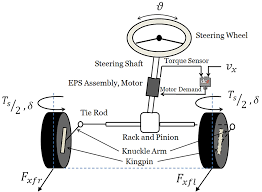
\includegraphics[height=1.5cm]{figs/img/autonomousVehiclesSteering}
				\caption{Autonomous Vehicle Steering System\textsuperscript{b}}
				\label{fig:steerSystem}
			\end{minipage}
        \end{figure}
    \begin{tiny}
		\textsuperscript{a}https://hexagonpositioning.com/pi-brands/autonomoustuff\\\textsuperscript{b}https://www.autonews.com/article/20181105/OEM10/181109921/delphi-s-pace-award-winning-e-steer-an-autonomous-vehicle-building-block
    \end{tiny}
\end{frame}

\begin{frame}{Problem Statement}
  \begin{block}{Problem Statement}
	\begin{minipage}[t]{0.62\linewidth}      
      Model different subsystems for an autonomous vehicle (Lexus RX450H platform is considered in this project), which are
	  \begin{multicols}{2}      
      \begin{itemize}
          \item Steering
          \item Acceleration
          \item Brake
          \item Shift
          \item Speed
          \item Speed control
        \end{itemize} 
        \end{multicols}
        using input-output raw data available offline
    \end{minipage}
    \begin{minipage}[t]{0.34\textwidth}  
        \begin{figure}
			\centering
			\captionsetup{justification=centering, margin=0.5cm, font=tiny}
			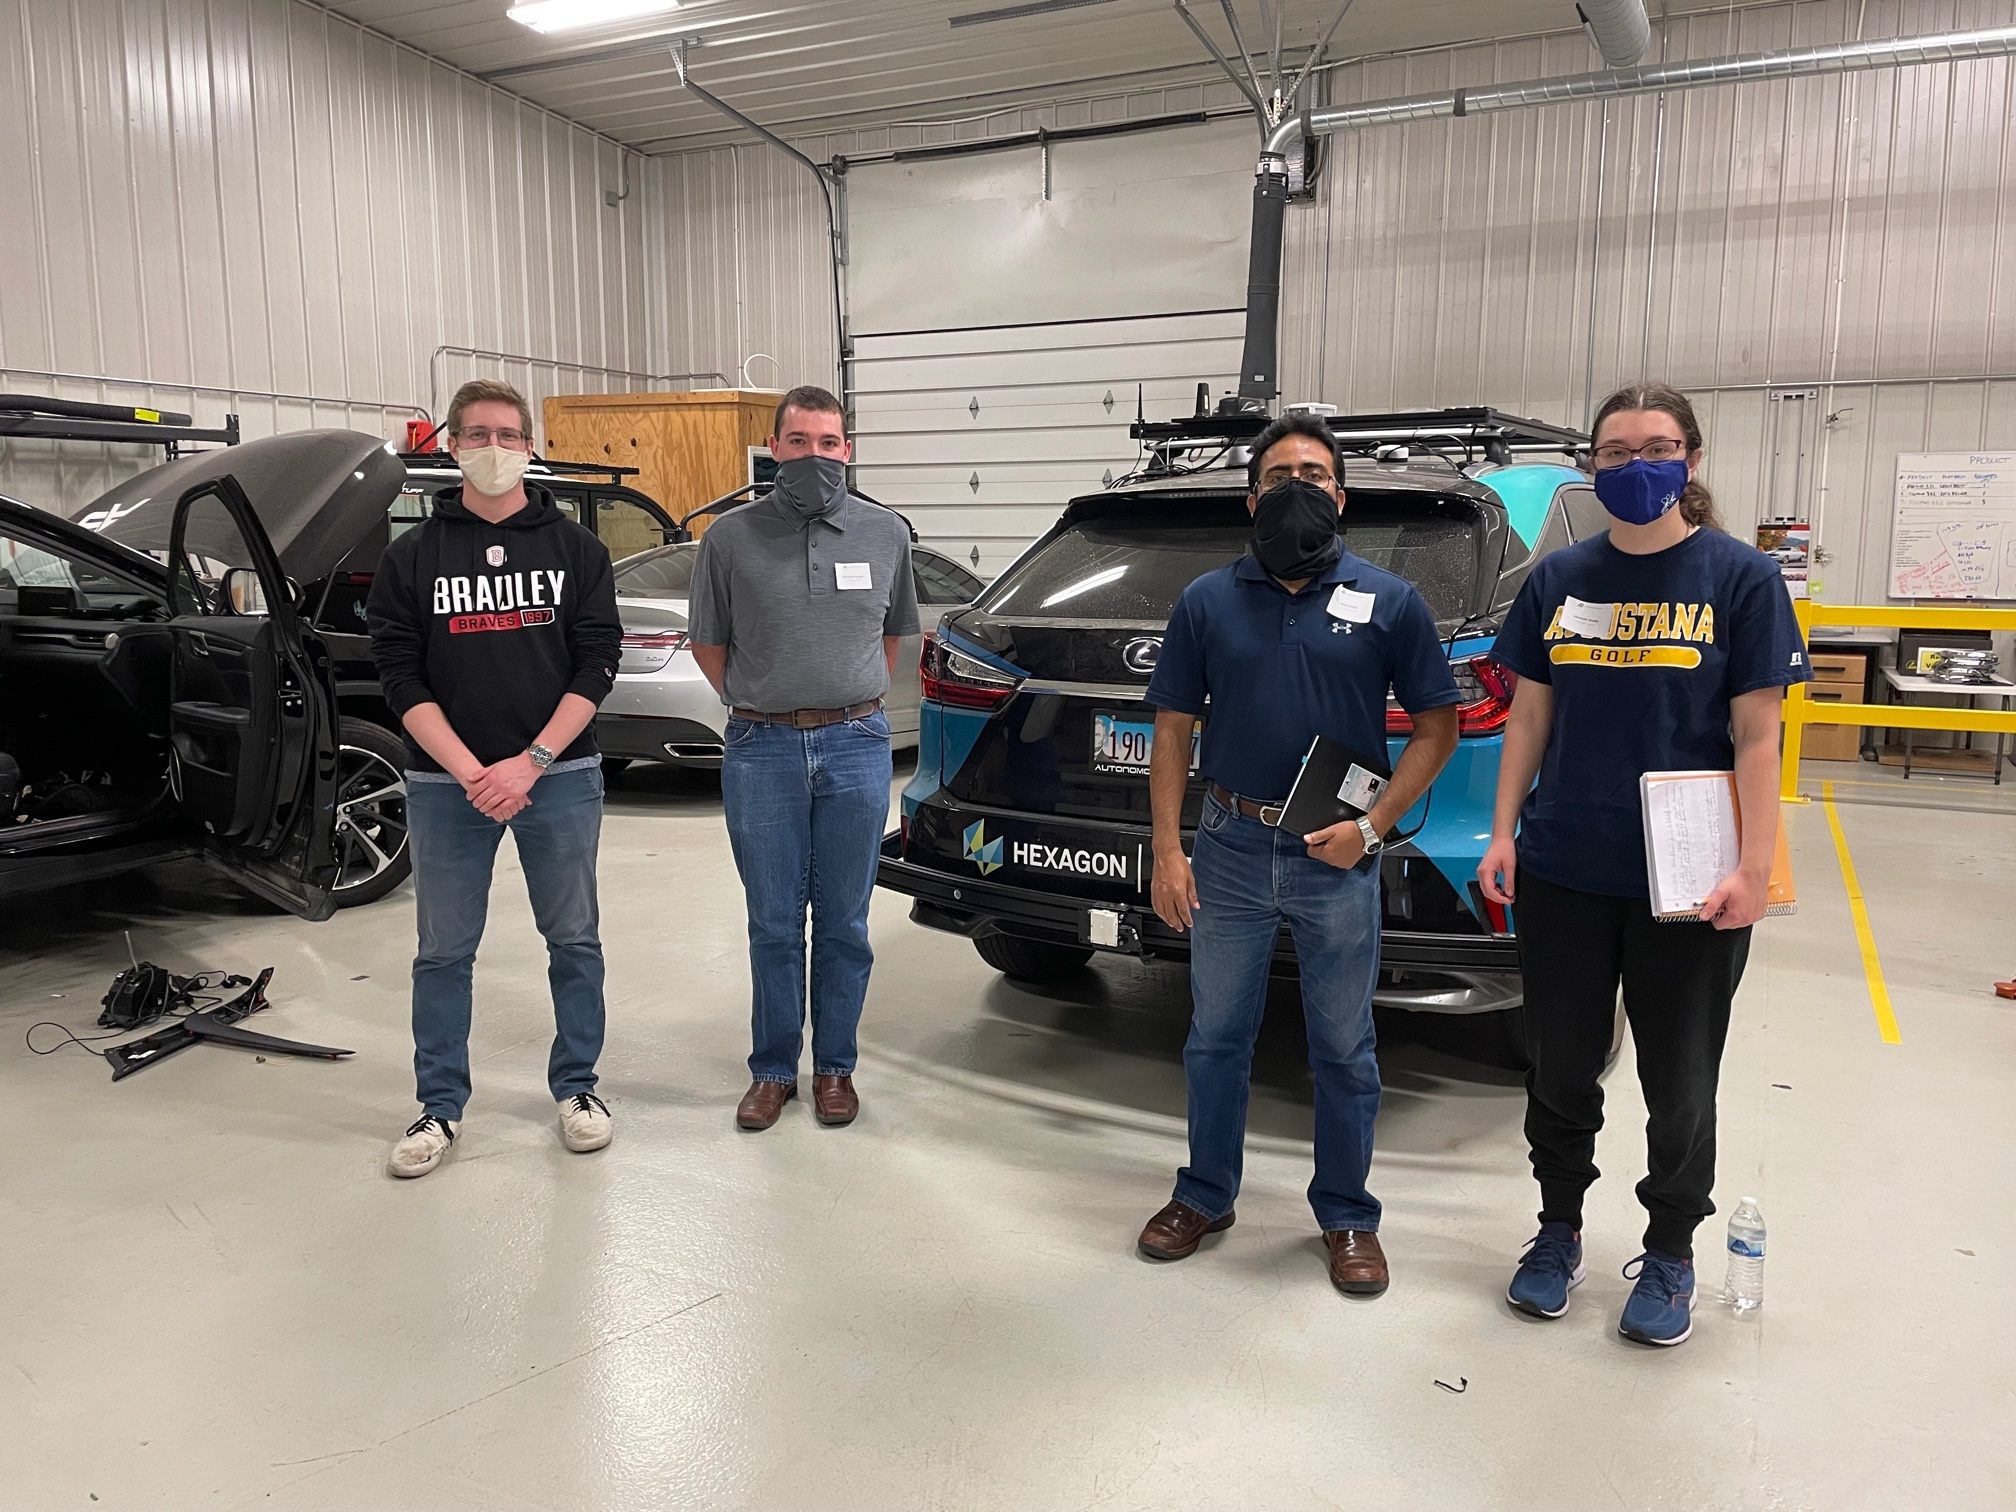
\includegraphics[width=4cm]{figs/img/picturesVisitToAStuff/visitors1-20211007}
			\caption{AutonomouStuff Lexus RX450H Vehicle}
		\end{figure}
	\end{minipage}
  \end{block}

  \pause
  \begin{block}{Proposed Solution}
    \begin{large}
      A potential solution is to develop conventional System Identification techniques for modeling subsystems using available raw data.  
    \end{large}
  \end{block}
\end{frame}

%----------------------------------

\section{Literature Review}

\begin{frame}{Literature Review}
  \begin{block}{Existing Solutions}
 \begin{itemize}
        \item Use of System Identification Toolbox in MATLAB to create models from data~\cite{Adnan2010}
	 \begin{itemize}
     \tiny
		    		\item Offers a variety of model choices
				\item Needs a large amount of raw data to produce an accurate model
	\end{itemize}
	\item Third order ARMAX model creates models using traditional methods of analysis~\cite{Li1999}
	 \begin{itemize}
     \tiny
		    		\item Allows the use of traditional analysis methods to create a model 
				\item More room for error during calculations
	\end{itemize}
	\item Steer-By-Wire method as a system model~\cite{Saruchi2015}
	 \begin{itemize}
     \tiny
		    		\item Can model systems with small non-linearities 
				\item Mechanical components replaced by electrical components 
	\end{itemize}
	\item Authors in~\cite{Hussain2011} illustrate identification of multiple-input single-output model for maximum power point tracking of photovoltaic system.  
	\begin{itemize}
    \tiny
		\item Fourth order ARX model ended up giving the best fit
	\end{itemize}
\end{itemize}
  \end{block}
    % \begin{figure}[b]
    %     \centering
    %     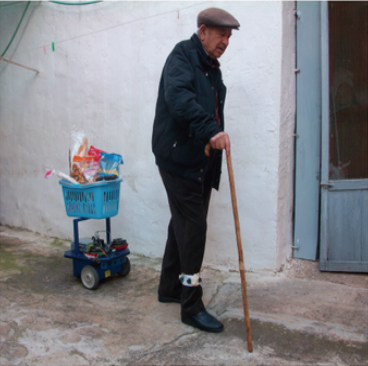
\includegraphics[width=0.45\textwidth]{figs/img/CompaRob}
    %     \caption{CompaRob}
    %     %\label{fig:sysBlockDiag}
    % \end{figure}
\end{frame}


%----------------------------------

\section{System Requirements}

\begin{frame}{System Requirements}
\begin{block}{Specifications}
	\begin{minipage}[t]{0.62\linewidth}    
    Proposed vehicle subsystem models are expected to fulfill requirements listed below:
	\begin{itemize}
    		\item Resulting plant model will consist of reasonably accurate subsystem models
    		\item Subsystems can be used to create a HIL testbench
    		\item Steering model can handle very small changes in steering angles
    \begin{itemize}
		\item smooth out any non-linear discontinuities that would normally be measured by the steering motor, especially for small changes in the steering angle, depicted in \autoref{fig:nonlinGraph}.
    \end{itemize}
	\end{itemize}
	\end{minipage}
	\begin{minipage}[t]{0.34\linewidth}
	\begin{figure}[h]
		\centering
    		\captionsetup{justification=centering, margin=0.5cm}
    		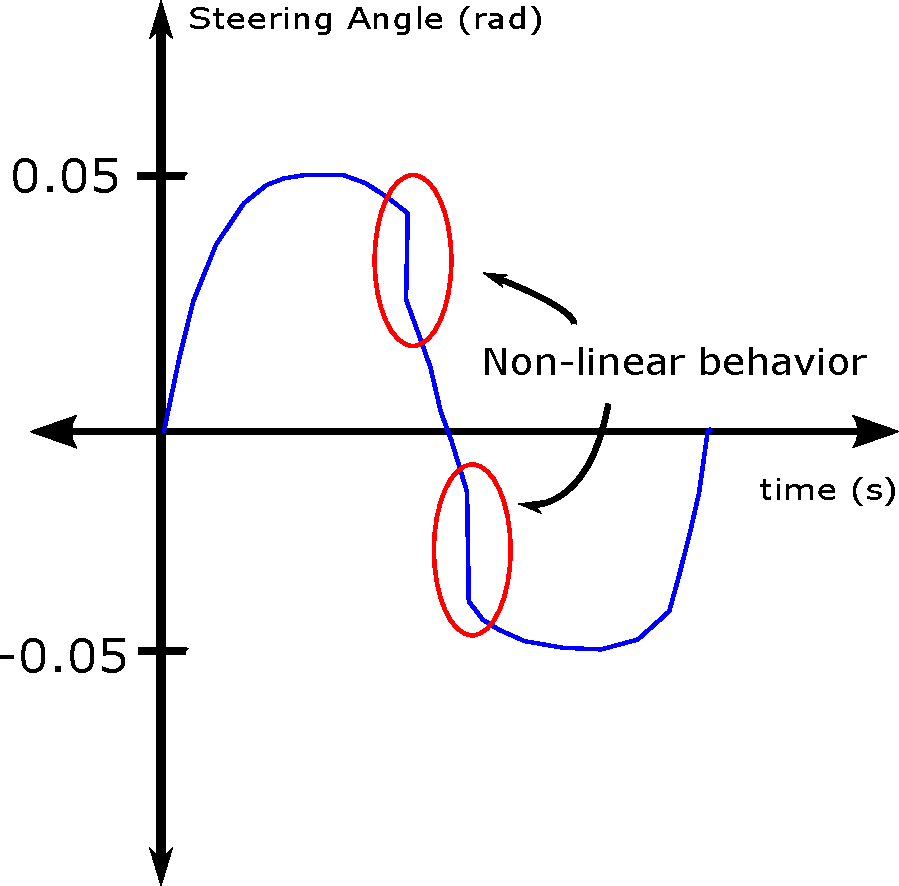
\includegraphics[width=1.5in]{figs/inkscape/nonlinearBehavior}
    		\caption{Steering Non-linear Behavior}
    		\label{fig:nonlinGraph}
	\end{figure}
	\end{minipage}
\end{block}
\end{frame}

%--------------------------------

\section{System Architecture}

\begin{frame}{System Architecture}
  \begin{block}{System Architecture}
    \begin{large}
      The overall system architecture of this project consists of six subsystems: 
      \begin{itemize}
          \item Steering
          \item Acceleration
          \item Brake %Model
          \item Shift %Model
          \item Speed %Model
          \item Speed control %Model
        \end{itemize} 
    \end{large}
  \end{block}
\end{frame}


\begin{frame}{System Architecture}
\centering \includegraphics[width=.45\linewidth]{figs/inkscape/steeringModelArchitecture}\quad%
\centering \begin{minipage}[b][0.4\textheight][c]{.45\linewidth} \begin{enumerate} \item Steering System \item Brake System \item Acceleration System \end{enumerate} \end{minipage}\\[1em]
\centering \includegraphics[width=.45\linewidth]{figs/inkscape/brakeModelArchitecture}\quad%
\centering 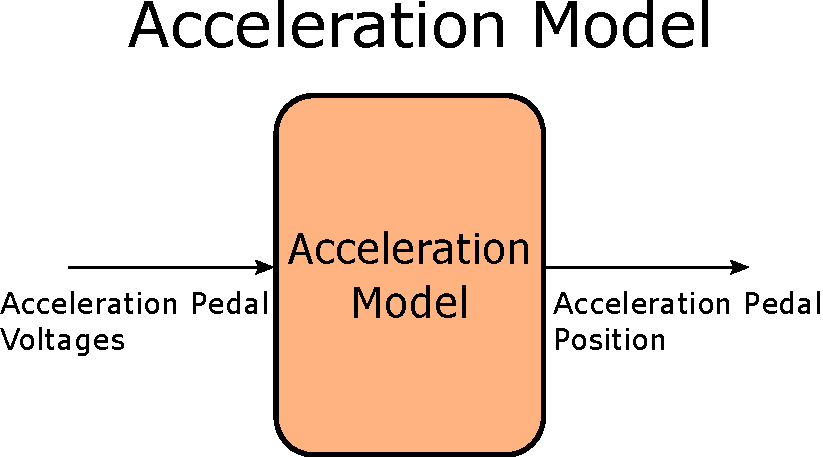
\includegraphics[width=.45\linewidth]{figs/inkscape/accelerationModelArchitecture}
\end{frame}


\begin{frame}{System Architecture}
\centering 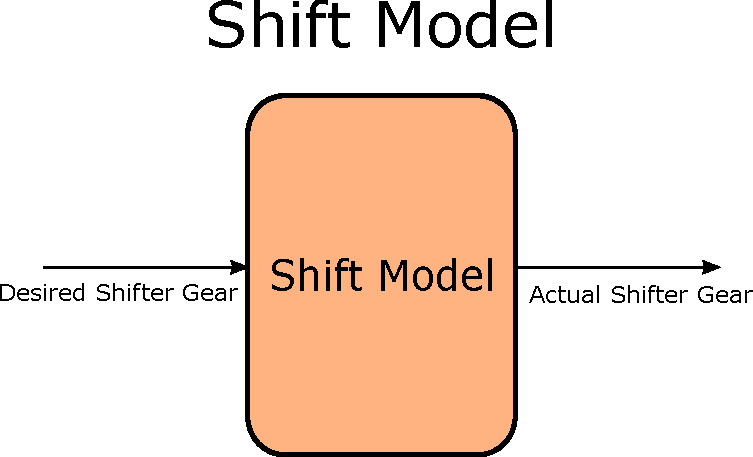
\includegraphics[width=.45\linewidth]{figs/inkscape/shiftModelArchitecture}\quad%
\centering \begin{minipage}[b][0.4\textheight][c]{.45\linewidth} \begin{enumerate} \item Shift System \item Speed Control System \item Speed System \end{enumerate} \end{minipage}\\[1em]
\centering \includegraphics[width=.45\linewidth]{figs/inkscape/speedControlModelArchitecture}\quad%
\centering \includegraphics[width=.45\linewidth]{figs/inkscape/speedModelArchitecture}
\end{frame}


\begin{frame}{System Architecture}
\begin{figure}[h]
    \centering
    \captionsetup{justification=centering, margin=3cm}
    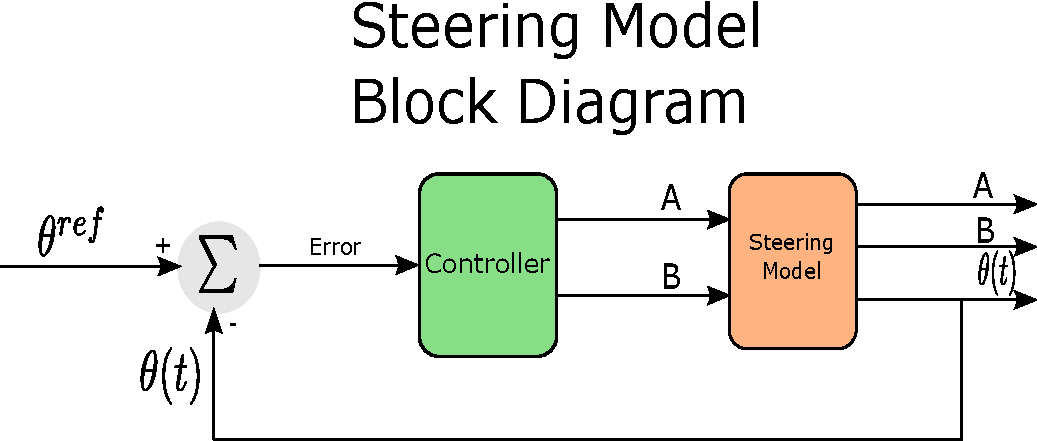
\includegraphics[width=4in]{figs/inkscape/steeringModelBlockDiagram}
    \caption{Steering System Block Diagram}
    \label{fig:steerBlockDiag}
\end{figure}
\end{frame}

\begin{frame}{System Inputs and Outputs}
\begin{minipage}[t]{0.48\linewidth}
\tiny
	\begin{block}{System Inputs}
		\begin{itemize}
			\tiny
		    \item Steering Model
		    \begin{itemize}
		    \tiny
		    		\item Torque Voltages
		    		\begin{itemize}
		    		\tiny
		    			\item Desired Steering Wheel Angle
		    			\item Actual Steering Wheel Angle
		    		\end{itemize}
		    \end{itemize}
		    \item Acceleration Model
		    \begin{itemize}
		    \tiny
		    		\item Acceleration Pedal Voltages
		    \end{itemize}
		    \item Brake Model
		    \begin{itemize}
		    \tiny
		    		\item Brake Pedal Pressure Voltages
		    		\item Brake Pedal Stroke Voltages 
		    		\item Brake Pedal On/Off Switch
		    \end{itemize}
		    \item Shift Model
		    \begin{itemize}
		    \tiny
		    		\item Desired Shift Gear
		    \end{itemize}
		    \item Speed Model
		    \begin{itemize}
		    \tiny
		    		\item Acceleration Pedal Position
		    		\item Brake Pedal Position
		    		\item Shifter Actual Gear
		    \end{itemize}
		    \item Speed Control Model
		    \begin{itemize}
		    \tiny
		    		\item Desired Vehicle Speed
		    \end{itemize}
		\end{itemize}
	\end{block}
\end{minipage}%
\hfill%
\begin{minipage}[t]{0.48\linewidth}
\begin{block}{System Outputs}
		\begin{itemize}
			\tiny
		    \item Steering Model
		    \begin{itemize}
		    \tiny
		    		\item Wheel Angle
		    		\item Actual Steering Angle
		    \end{itemize}
		    \item Acceleration Model
		    \begin{itemize}
		    \tiny
		    		\item Acceleration Pedal Position
		    \end{itemize}
		    \item Brake Model
		    \begin{itemize}
		    \tiny
		    		\item Brake Pedal Position
		    		\item Brake Pressed
		    \end{itemize}
		    \item Shift Model
		    \begin{itemize}
		    \tiny
		    		\item Actual Shift Gear
		    \end{itemize}
		    \item Speed Model
		    \begin{itemize}
		    \tiny
		    		\item Vehicle Speed
		    \end{itemize}
		    \item Speed Control Model
		    \begin{itemize}
		    \tiny
		    		\item Vehicle Speed
		    \end{itemize}
		\end{itemize}
	\end{block}
\end{minipage}
\end{frame}

%----------------------------------

\section{System Identification}

\begin{frame}{System Identification}
  \begin{block}{System Identification}
 \begin{itemize}
        \item Developing mathematical models for a dynamic system
        \item Uses the measurement of the input and output signals
        \begin{itemize}
        		\item Single Input Single Output (SISO)
        		\item Single Input Multiple Output (SIMO)
        		\item Multiple Input Single Output (MISO)
        		\item Multiple Input Multiple Output (MIMO)
        \end{itemize}
        \item Achieve an accurate estimation of the system response for any given input
        \item Mathworks' MATLAB System Identification Toolbox
\end{itemize}
  \end{block}
\end{frame}

\subsection{Preliminary Work}

\begin{frame}{Preliminary Work}
  \begin{block}{Preliminary Work}
 \begin{itemize}
        \item Documentation on MATLAB's System Identification Toolbox and tutorials
        \item Literature Review 
        \item Data Collection for steering, braking and acceleration subsystems
\end{itemize}
  \end{block}
  
   \begin {block}{MATLAB Example: Dealing with Multi-Variable Systems: Identification and Analysis}
  \begin{itemize}
  	\item  Learned how to create an iddata object from a given data set 
  	\item Created a state space model and compared it to the validation data 
  	\item Tried creating submodels for some of the channels in order to try and get a better fit 
  	\item Then created a MISO model and learned how to merge the two SISO models that were created earlier 
  	\end{itemize}
  	\end{block}

\end{frame}

%----------------------------------
\subsection{Experimental Setup}

\begin{frame}{Experimental Setup}
	\begin{block}{Control Method}
		\begin{itemize}
			\item Manual Mode
			\begin{itemize}
				\item Vehicle is not autonomous
				\item Torque voltages are sent by the vehicle ECU
			\end{itemize}
			\item By-Wire Mode
			\begin{itemize}
				\item Vehicle is autonomous
				\item Torque voltages are sent by the PACMod ECU
				\item Torque voltages sent from the vehicle ECU are discarded by open-circuiting the motors
			\end{itemize}
		\end{itemize}
		\begin{figure}
			\centering
    			\captionsetup{justification=centering, margin=3cm}
    			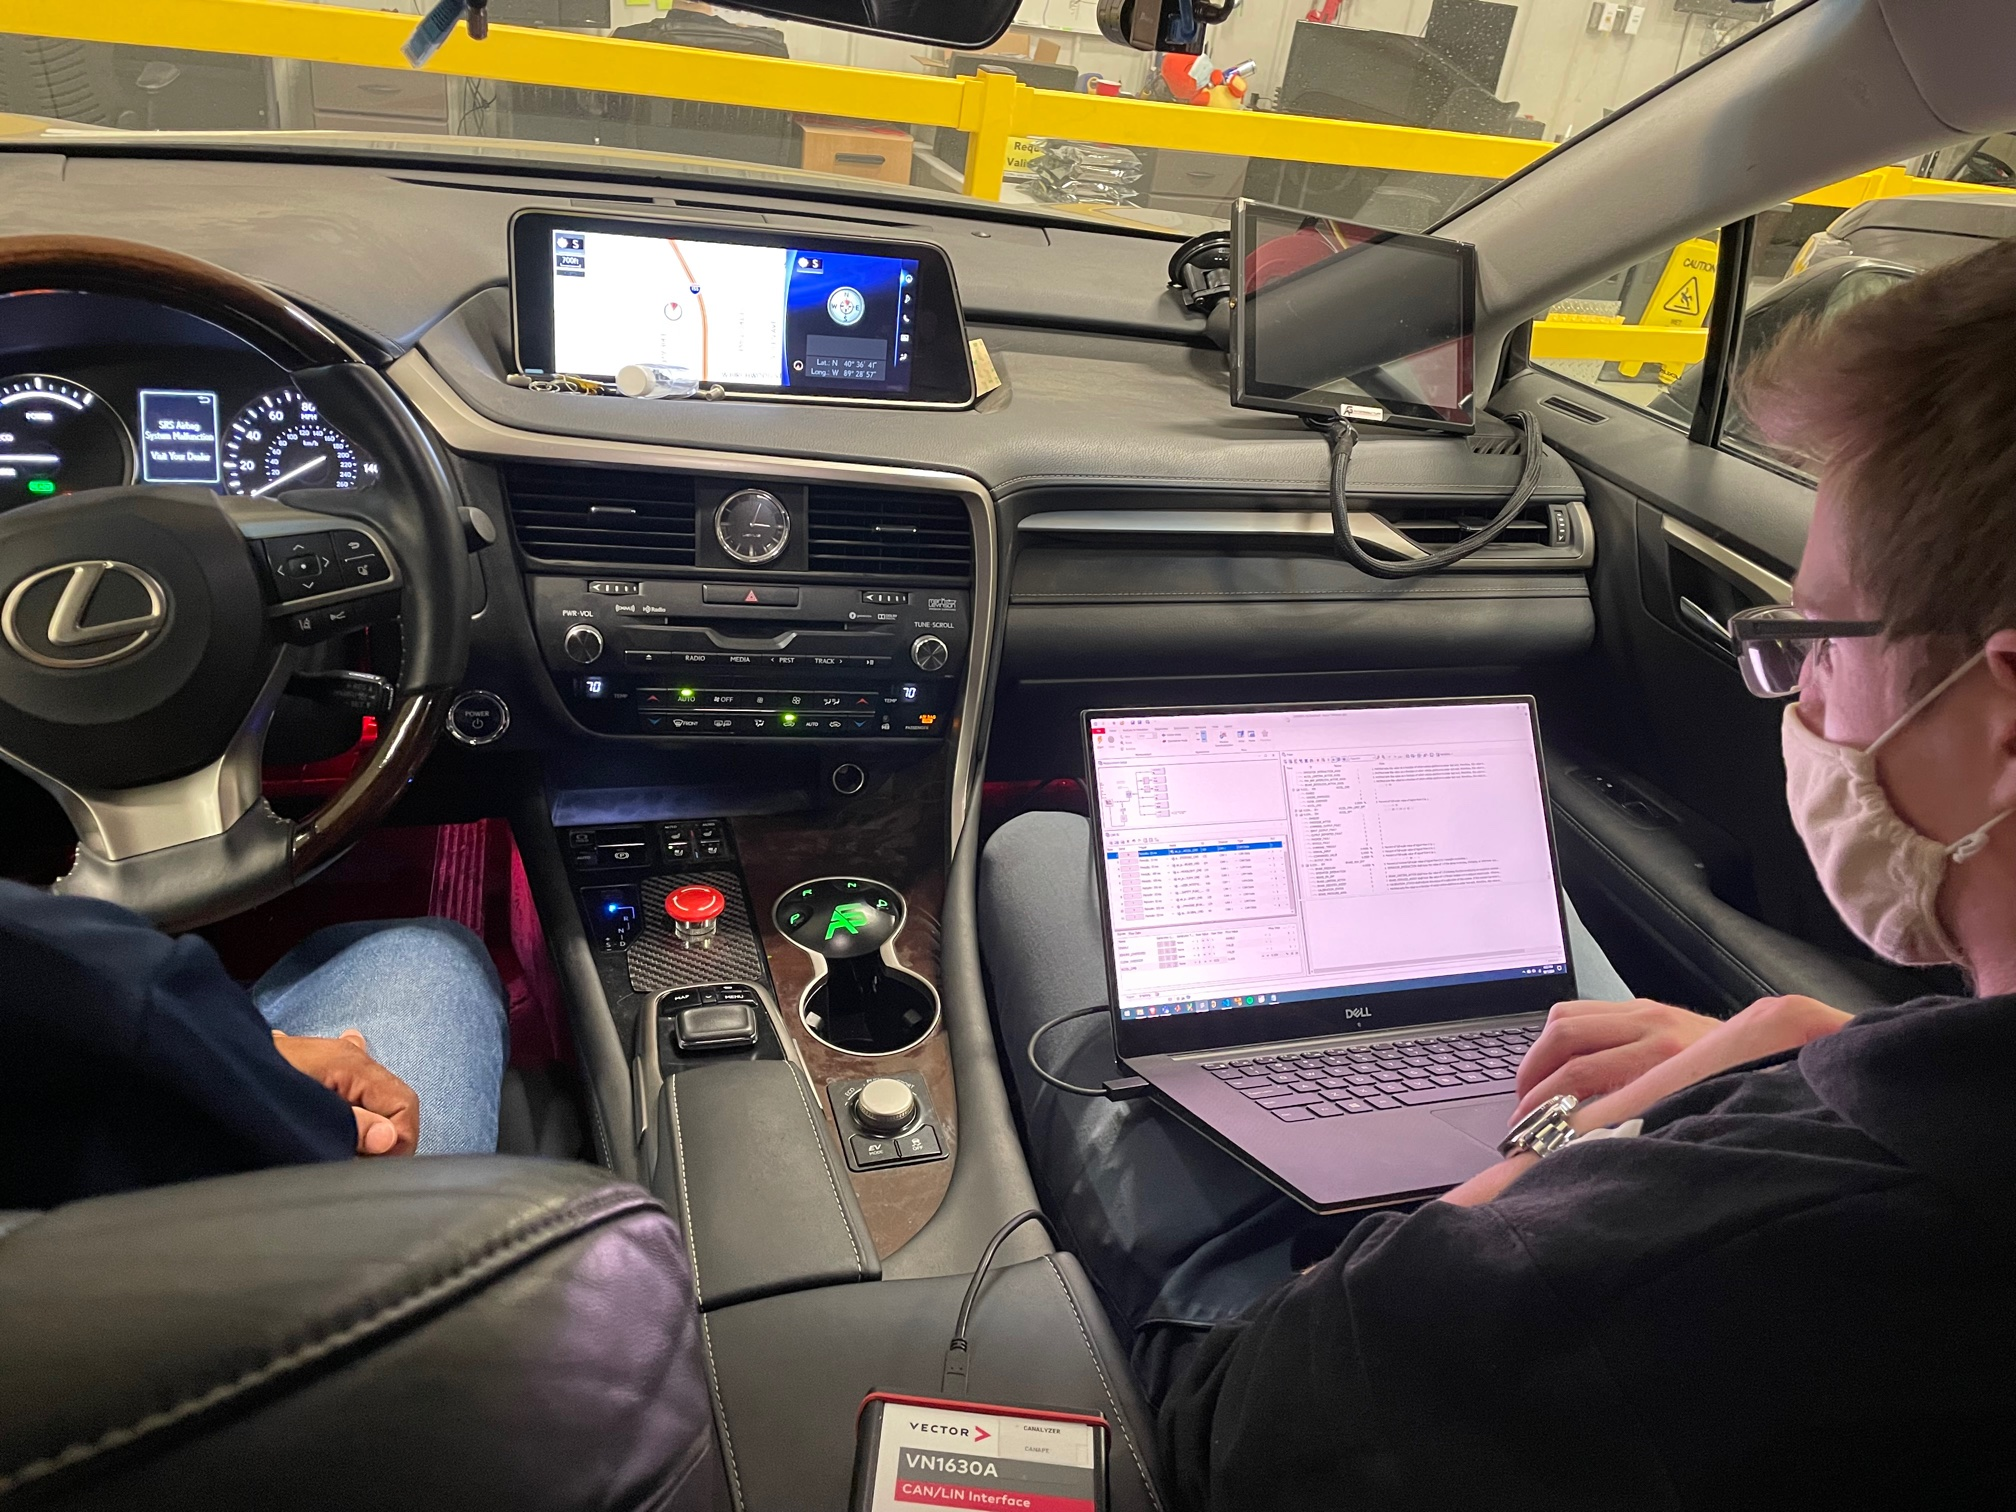
\includegraphics[width=1in]{figs/img/picturesVisitToAStuff/dataColletionSetup1-20211007}
    			\caption{Autonomous Vehicle Data Collection Setup}
    			\label{fig:vehicleSetup}
		\end{figure}
	\end{block}
\end{frame}

%----------------------------------
\subsection{Parts List}

\begin{frame}{Parts List}
  \begin{block}{Software and Hardware}
 \begin{itemize}
        \item Software
        \begin{itemize}
        \small
        \item MATLAB's System Identification Toolbox
        \item Vector CANAlyzer
        \end{itemize}
	\item Hardware
	\begin{itemize}
	\small
	\item Laptop
	\item PACMod ECU
	\item CANCase 
	\item CAN bus
	\end{itemize}
\end{itemize}
  \end{block}
\end{frame}

%----------------------------------
\subsection{Modeling}

\begin{frame}{Model Equations}
	\begin{block}{Model Equations}
		\begin{itemize}
			\item Transfer Function Model: 
			\begin{equation}
				\frac{Y(s)}{U_A(s)} = \frac{b_{n}s^{n} + b_{n-1}s^{n-1} + ... + b_1s + b_0}{a_{m}s^{m} + a_{m-1}s^{m-1} + ... + a_1s + a_0}
			\end{equation}
			where m = number of poles and n = number of zeros
			\item ARX Model: 
			\begin{equation}
				A(z)y(t) = B(z)u(t) + e(t)
			\end{equation}
		\end{itemize}
	\end{block}
\end{frame}

\begin{frame}{Model Equations}
	\tiny	
	\begin{block}{ARX Model MATLAB Representation}
		The polynomial equation for an ARX Model is:
		\begin{equation}
			y(t) + a_1y(t - 1) +...+a_{na}y(t - n_{a}) = b_{1}u(t-n_{k})+...+b_{nb}u(t - n_{k}-n_{b}+1) + e(t)
		\end{equation}
		where na, nb, and nk are the system’s number of poles, number of zeros, and the system dead time, respectively
		MATLAB represents the ARX Model with the following equation:
		\begin{equation}
			A(z)y(t) = B(z)u(t - n_k) + e(t)
		\end{equation}
		where z is a delay operator and 
		\begin{equation}
			A(z) = 1 + a_1z^{-1} + ... + a_{na}z^{-n_a}
		\end{equation}
		\begin{equation}
			B(z) = b_1 + b_2z^{-1} + ... + b_{nb}z^{-n_b}
		\end{equation}
		For MISO systems, MATLAB uses the following equation to represent the ARX Model:
		\begin{equation}
			A(z)y(t) = B_1(z)u_1(t - nk_{1}) + B_2(z)u_2(t - nk_{2}) + ... + B_{nu}(z)u_{nu}(t - nk_{nu})
		\end{equation}
		where nu is the number of system inputs
	\end{block}
\end{frame}

%----------------------------------
\section{Validation and Testing}

\begin{frame}{Simulation Results}
  \begin{block}{Steering System}
 \begin{itemize}
	\item Best fit percentage of the by-wire steering estimated model is 85.54
	\item Best fit percentage of the manual steering estimated model is 90.27
 \end{itemize}
 \begin{figure}
    \centering
    \begin{minipage}{0.45\textwidth}
        \centering
        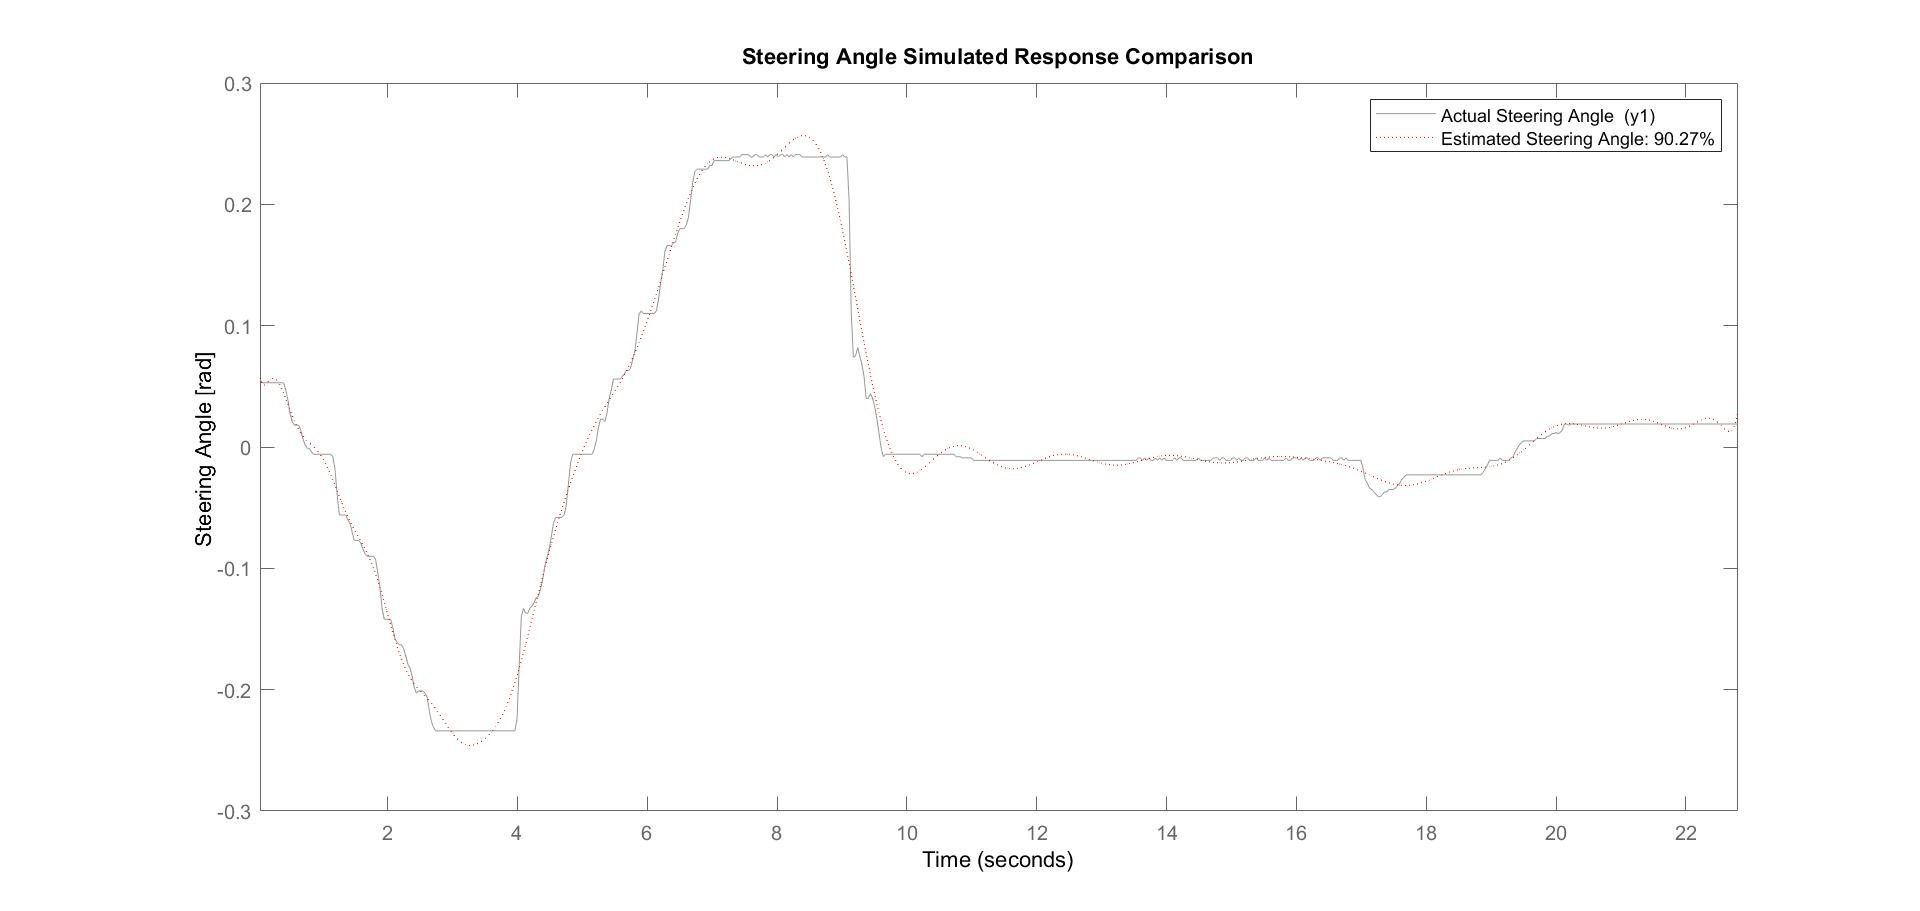
\includegraphics[width=0.6\textwidth]{figs/img/byWireSteeringTransferFunctionModel} % first figure itself
        \caption{Output of Estimated By-Wire System Model}
        \label{fig:byWireSteerModel}
    \end{minipage}\hfill
    \begin{minipage}{0.45\textwidth}
        \centering
        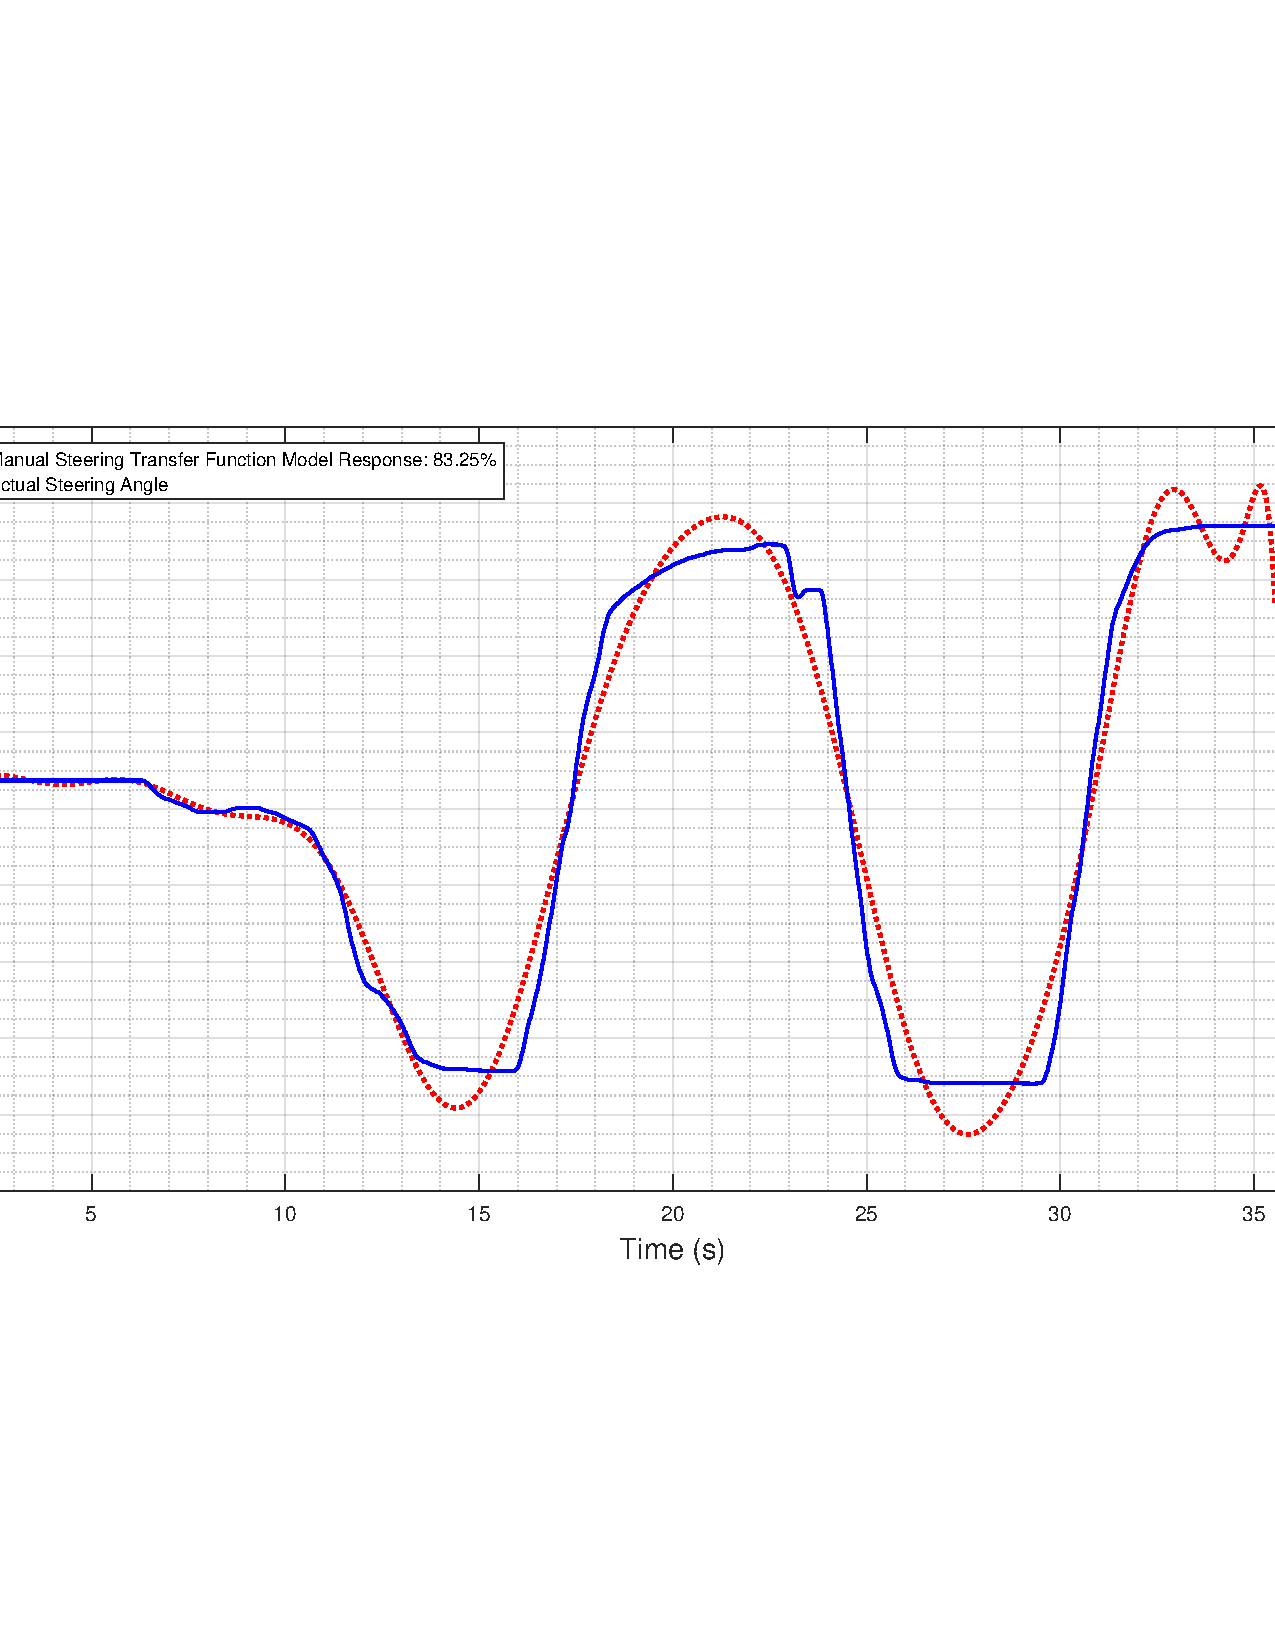
\includegraphics[width=0.6\textwidth]{figs/img/manualSteeringTransferFunctionModel} % second figure itself
        \caption{Output of Estimated Manual System Model}
        \label{fig:manualSteerModel}
    \end{minipage}
\end{figure}
  \end{block}
\end{frame}

\begin{frame}{By-Wire Steering System Transfer Function}

\begin{block}{Torque Voltage A}
	  \resizebox{\linewidth}{!}{% Resize table to fit within \linewidth horizontally
    \begin{tabular}{*{21}{c}}
      \toprule
      $a_0$& $a_1$&$a_2$&$a_3$&$a_4$&$a_5$&$a_6$&$a_7$&$a_8$&$a_9$&$a_{10}$&$a_{11}$&$a_{12}$&$a_{13}$&$a_{14}$&$a_{15}$&$a_{16}$&$a_{17}$&$a_{18}$ &$a_{19}$&$a_{20}$\\
      \midrule
      1.949E-16 & 1.455E-14 & 8.797E-13 & 2.304E-11 & 9.041E-10 & 9.01E-9 & 2.714E-7 & 9.241E-7 & 1.946E-5 & 3.889E-5 & 0.0005721 & 0.0008035 & 0.008695 & 0.008922 & 0.07499 & 0.05422 & 0.3631 & 0.1693 & 0.9394 & 0.2118 & 1\\
      \bottomrule
    \end{tabular}}
    
	\begin{center}
		\resizebox{0.4\linewidth}{!}{% Resize table to fit within \linewidth horizontally
    		\begin{tabular}{*{21}{c}}
      	\toprule
      	$b_0$& $b_1$&$b_2$&$b_3$&$b_4$&$b_5$\\
      	\midrule
      	3.44E-16 & -2.203E-15 & 1.24E-13 & 5.975E-13 & 3.001E-12 & 5.23E-12\\
      	\bottomrule
    		\end{tabular}}
	\end{center}	    

\end{block}
\begin{block}{Torque Voltage B}
	  \resizebox{\linewidth}{!}{% Resize table to fit within \linewidth horizontally
    \begin{tabular}{*{21}{c}}
      \toprule
      $a_0$& $a_1$&$a_2$&$a_3$&$a_4$&$a_5$&$a_6$&$a_7$&$a_8$&$a_9$&$a_{10}$&$a_{11}$&$a_{12}$&$a_{13}$&$a_{14}$&$a_{15}$&$a_{16}$&$a_{17}$&$a_{18}$ &$a_{19}$&$a_{20}$\\
      \midrule
      2.92E-15 & 2.758E-13 & 1.761E-11 & 4.228E-10 & 1.422E-8 & 1.561E-7 & 1.501E-6 & 8.426E-6 & 5.981E-5 & 0.0002016 & 0.001226 & 0.002649 & 0.01456 & 0.02044 & 0.104 & 0.09228 & 0.4417 & 0.2257 & 1.025 & 0.2305 & 1\\
      \bottomrule
    \end{tabular}}
	\begin{center}
		\resizebox{0.4\linewidth}{!}{% Resize table to fit within \linewidth horizontally
    		\begin{tabular}{*{21}{c}}
     	 \toprule
     	 $b_0$& $b_1$&$b_2$&$b_3$&$b_4$&$b_5$\\
     	 \midrule
      	-6.645E-15 & 2.161E-14 & -2.605E-14 & -4.744E-13 & -1.813E-13 & -4.858E-12\\
      	\bottomrule
    \end{tabular}}
	\end{center}	    	 
\end{block}  
\end{frame}


\begin{frame}{Manual Steering System Transfer Function}

\begin{block}{Torque Voltage A}
	  \resizebox{\linewidth}{!}{% Resize table to fit within \linewidth horizontally
    \begin{tabular}{*{21}{c}}
      \toprule
      $a_0$& $a_1$&$a_2$&$a_3$&$a_4$&$a_5$&$a_6$&$a_7$&$a_8$&$a_9$&$a_{10}$&$a_{11}$&$a_{12}$&$a_{13}$&$a_{14}$&$a_{15}$&$a_{16}$&$a_{17}$&$a_{18}$ &$a_{19}$&$a_{20}$\\
      \midrule
      1.224E5 & 4.227E5 & 2.202E6 & 3.54E6 & 7.98E6 & 7.62E5 & 1.071E7 & 6.745E6 & 6.85E6 & 3.006E6 & 2.365E6 & 7.37E5 & 4.669E5 & 1.021E5 & 5.319E4 & 7752 & 3353 & 287.5 & 102.4 & 3.653 & 1\\
      \bottomrule
    \end{tabular}}
    \begin{center}
    	\resizebox{0.4\linewidth}{!}{% Resize table to fit within \linewidth horizontally
    \begin{tabular}{*{21}{c}}
      \toprule
      $b_0$& $b_1$&$b_2$&$b_3$&$b_4$&$b_5$\\
      \midrule
      6.516E4 & -2.944E5 & 2.328E5 & -2.487E5 & 8.25E4 & -3.038E4\\
      \bottomrule
    \end{tabular}}
    \end{center}
\end{block}
\begin{block}{Torque Voltage B}
	  \resizebox{\linewidth}{!}{% Resize table to fit within \linewidth horizontally
    \begin{tabular}{*{21}{c}}
      \toprule
      $a_0$& $a_1$&$a_2$&$a_3$&$a_4$&$a_5$&$a_6$&$a_7$&$a_8$&$a_9$&$a_{10}$&$a_{11}$&$a_{12}$&$a_{13}$&$a_{14}$&$a_{15}$&$a_{16}$&$a_{17}$&$a_{18}$ &$a_{19}$&$a_{20}$\\
      \midrule
      4.687E4 & 7.037E5 & 2.624E6 & 6.133E6 & 1.197E7 & 1.487E7 & 1.887E7 & 1.446E7 & 1.314E7 & 7.01E6 & 4.79E6 & 1.886E6 & 9.836E5 & 2.937E5 & 1.149E5 & 2.617E4 & 7205 & 1232 & 200 & 23.54 & 1\\
      \bottomrule
    \end{tabular}}
	\begin{center}
	\resizebox{0.4\linewidth}{!}{% Resize table to fit within \linewidth horizontally
    \begin{tabular}{*{21}{c}}
      \toprule
      $b_0$& $b_1$&$b_2$&$b_3$&$b_4$&$b_5$\\
      \midrule
      1.209E4 & 1.855E5 & -2.801E5 & 4.72E5 & -3.976E4 & 7.693E4\\
      \bottomrule
    \end{tabular}}
	\end{center}	    	  
\end{block}
\end{frame}


\begin{frame}{Simulation Results}
  \begin{block}{Acceleration System}
 \begin{itemize}
	\item Best fit percentage of the by-wire acceleration estimated model is 97.69
	\item Best fit percentage of the manual acceleration estimated model is 98.3
 \end{itemize}
 \begin{figure}
    \centering
    \begin{minipage}{0.45\textwidth}
        \centering
        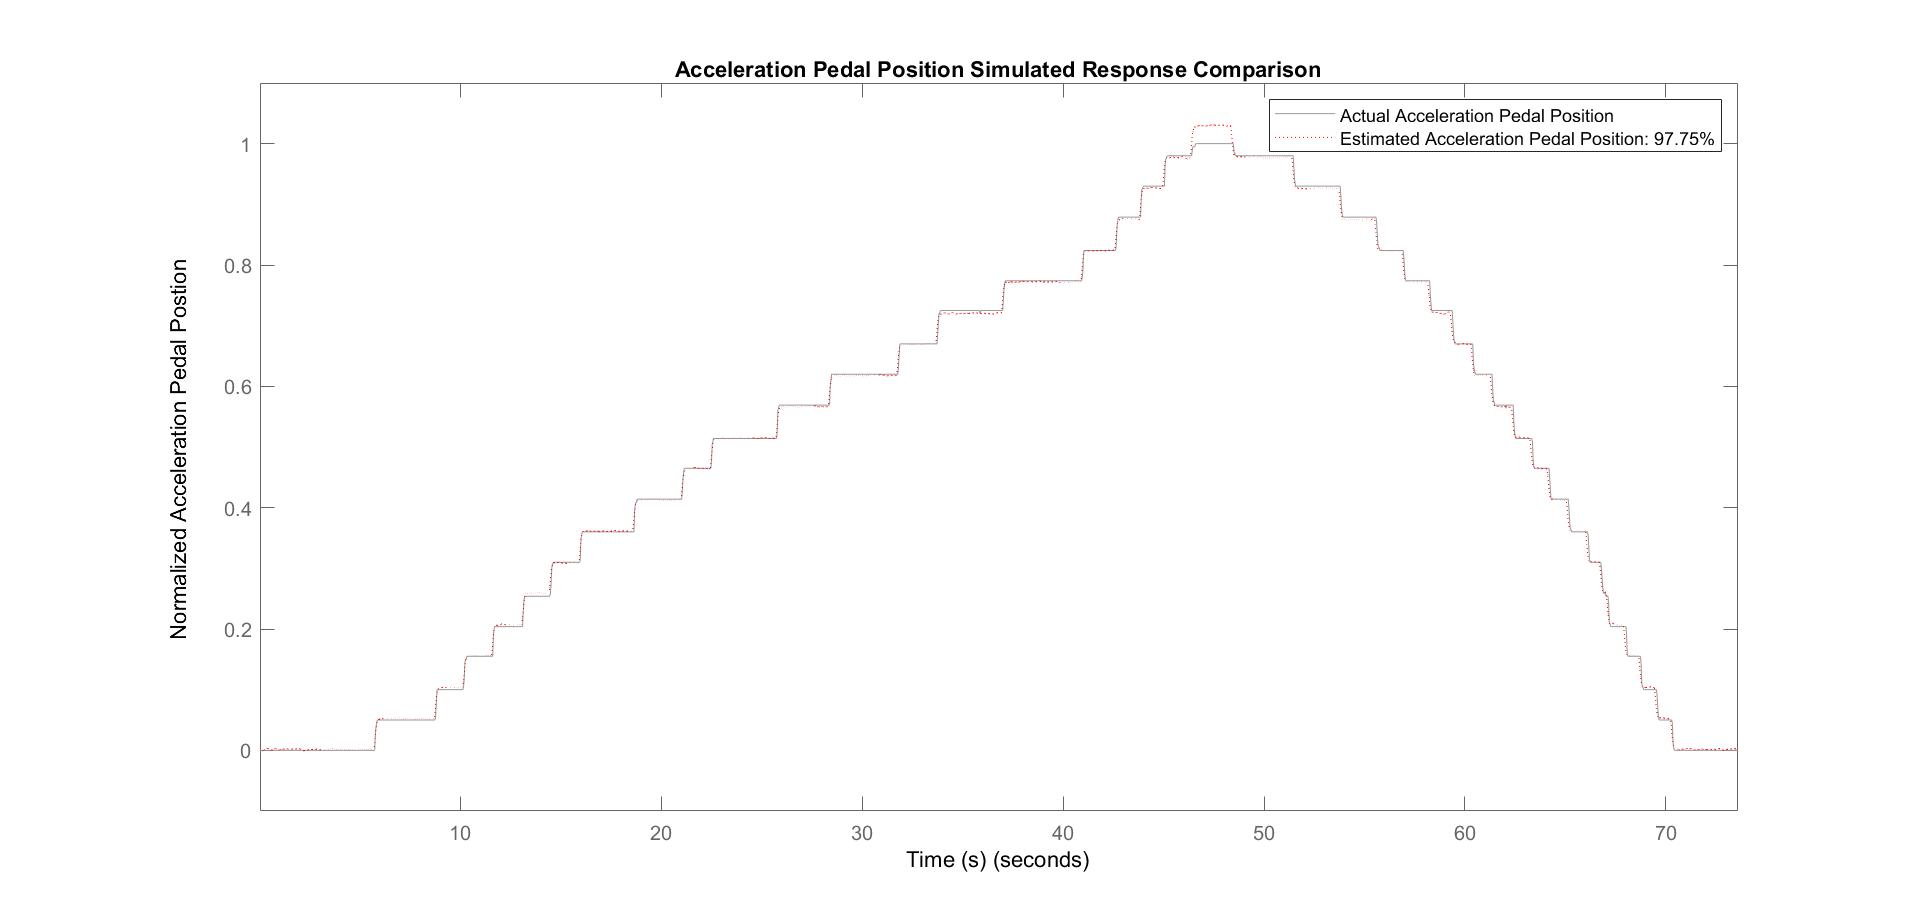
\includegraphics[width=0.6\textwidth]{figs/img/byWireAccelArxModel} % first figure itself
        \caption{Output of Estimated By-Wire System Model}
        \label{fig:byWireAccelModel}
    \end{minipage}\hfill
    \begin{minipage}{0.45\textwidth}
        \centering
        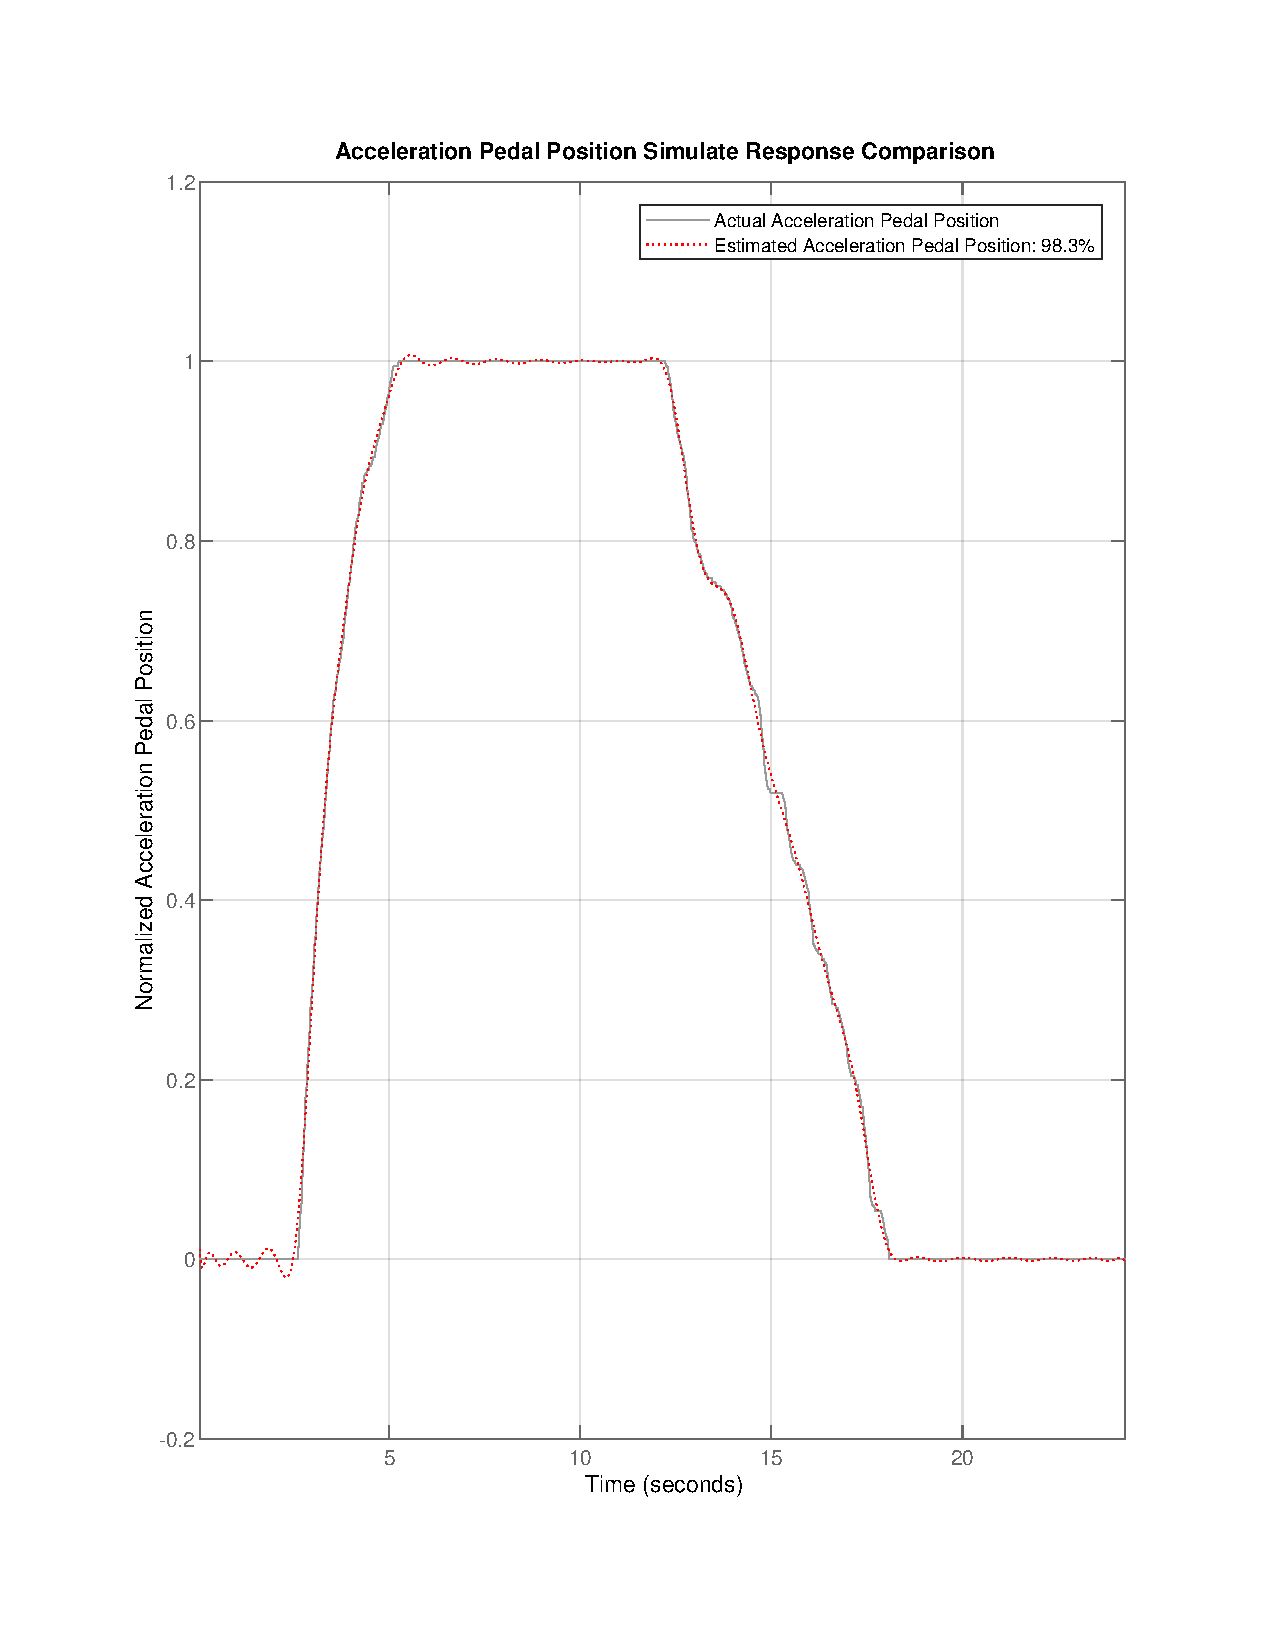
\includegraphics[width=0.6\textwidth]{figs/img/manualAccelTransferFunctionModel} % second figure itself
        \caption{Output of Estimated Manual System Model}
        \label{fig:manualAccelModel}
    \end{minipage}
\end{figure}
  \end{block}
\end{frame}

\begin{frame}{By-Wire Acceleration System Transfer Function}
	\begin{block}{Fourth-Order ARX Model}
		\begin{equation}
			A(z)y(t) = B_1(z)u_1(t) + B_2(z)u_2(t) + e(t)
		\end{equation}
		%
		\centering where na = 4, nb = 4, nk = 0, and, 
		%
		\begin{equation}
			A(z) = 1 - 1.018z^{-1} - 0.002901z^{-2} + 0.4631z^{-3} - 0.2038z^{-4}
		\end{equation}
		\begin{equation}
			B_1(z) = -0.0207 - 0.01912z^{-1} - 0.02159z^{-2} - 0.03307z^{-3}
		\end{equation}
		\begin{equation}
			B_2(z) = 0.02017 + 0.01833z^{-1} + 0.09461z^{-2} + 0.05683z^{-3}
		\end{equation}
	\end{block}
\end{frame}

\begin{frame}{Manual Acceleration System Transfer Function}
\begin{block}{Torque Voltage A}
	  \resizebox{\linewidth}{!}{% Resize table to fit within \linewidth horizontally
    \begin{tabular}{*{25}{c}}
      \toprule
      $a_0$& $a_1$&$a_2$&$a_3$&$a_4$&$a_5$&$a_6$&$a_7$&$a_8$&$a_9$&$a_{10}$&$a_{11}$&$a_{12}$&$a_{13}$&$a_{14}$&$a_{15}$&$a_{16}$&$a_{17}$&$a_{18}$ &$a_{19}$&$a_{20}$&$a_{21}$&$a_{22}$&$a_{23}$&$a_{24}$\\
      \midrule
      2.307E7 & 8.369E7 & 9.137E8 & 1.992E9 & 3.753E9 & 5.454E9 & 5.548E9 & 5.869E9 & 3.453E9 & 3.161E9 & 1.54E9 & 9.654E8 & 3.556E8 & 1.789E8 & 5.082E7 & 2.071E7 & 4.569E6 & 1.498E6 & 2.553E5 & 6.532E4 & 8443 & 1559 & 147.3 & 15.5 & 1\\
      \bottomrule
    \end{tabular}}
    \begin{center}
    		\resizebox{0.4\linewidth}{!}{% Resize table to fit within \linewidth horizontally
    \begin{tabular}{*{7}{c}}
      \toprule
      $b_0$& $b_1$&$b_2$&$b_3$&$b_4$&$b_5$&$b_6$\\
      \midrule
      -5.741E6 & -2.644E7 & -2.797E6 & -1.304E7 & -3.203E6 & -1.159E6 & -5.519E5\\
      \bottomrule
    \end{tabular}}
    \end{center}
\end{block}
\begin{block}{Torque Voltage B}
	  \resizebox{\linewidth}{!}{% Resize table to fit within \linewidth horizontally
    \begin{tabular}{*{25}{c}}
      \toprule
      $a_0$& $a_1$&$a_2$&$a_3$&$a_4$&$a_5$&$a_6$&$a_7$&$a_8$&$a_9$&$a_{10}$&$a_{11}$&$a_{12}$&$a_{13}$&$a_{14}$&$a_{15}$&$a_{16}$&$a_{17}$&$a_{18}$ &$a_{19}$&$a_{20}$&$a_{21}$&$a_{22}$&$a_{23}$&$a_{24}$\\
      \midrule
      5.224E6 & 4.205E7 & 1.429E8 & 3.233E8 & 5.444E8 & 7.326E8 & 8.247E8 & 7.402E8 & 6.301E8 & 3.99E8 & 2.731E8 & 1.264E8 & 7.223E7 & 2.48E7 & 1.216E7 & 3.084E6 & 1.324E6 & 2.422E5 & 9.264E4 & 1.159E4 & 4003 & 307.4 & 96.87 & 3.451 & 1\\
      \bottomrule
    \end{tabular}}
    \begin{center}
    	\resizebox{0.4\linewidth}{!}{% Resize table to fit within \linewidth horizontally
    \begin{tabular}{*{7}{c}}
      \toprule
      $b_0$& $b_1$&$b_2$&$b_3$&$b_4$&$b_5$&$b_6$\\
      \midrule
      -4.159E6 & 1.851E6 & -4.457E6 & 9.043E5 & -7.45E5 & 1.865E5 & -1.545E4\\
      \bottomrule
    \end{tabular}}
    \end{center}
\end{block}
\end{frame}


%----------------------------------
\section{Timeline and Milestones}

\begin{frame}{Timeline and Milestones}
  \begin{block}{Milestones}
 \begin{itemize}
        \item Model steering subsystem 
	\item Test subsystem models with HIL system 
	\item Final report and presentation 
\end{itemize}
  \end{block}
  
  \begin{block}{Timeline}
  \begin{itemize}
  \item Fall Semester
  \begin{itemize}
	\begin{tiny}
	\item System Identification Documentation 
	\item Collect Steering, Acceleration, and Brake Data 
	\item System Identification Tutorials
	\item System Functional Requirements Document and Presentation
	\item Proposal Document and Presentation 
	\item Model Steering, Acceleration, and Brake Subsystems 
	\end{tiny}
	\end{itemize}
	\item Spring Semester
	\begin{itemize}
	\begin{tiny}
	\item Collect Shift, Speed Control, and Speed Data  
	\item Model Shift, Speed Control, and Speed Subsystems  
	\item Test Subsystems
	\item Test Subsystems with HIL
	\item Final Report and Presentation 
	\item IAB Presentation 
	\item Project Demonstration  
	\end{tiny}
	\end{itemize}
	\end{itemize}
  \end{block}
   


\end{frame}


%----------------------------------

%\begin{frame}{Other Considerations}
%  \begin{block}{Factors}
%  	\begin{small}
%      \begin{itemize}
%        \item Public Health: Autonomous vehicles can make roads safer, which can prevent accidents
%and driving fatalities and injuries. As a result, people will be able to live longer and
%healthier lives. By creating accurate models, we will help advance the development of
%autonomous vehicles and make this a reality.
%		\item Public Safety: This is a relevant concern, because the real world implementations of inaccurate models could be disastrous since it is a self-driving vehicle. We will address this by creating a rigorous test plan for our models.
%		\item Public Welfare: This factor is somewhat related to public safety and health in that we need to make sure that these vehicles are safe for people to use. How we will help
%ensure this in our project is the same as how we will ensure public safety, by making sure we throughly test our models.
%		\item Global Factors: 
%		\item Cultural Factors: 
%		\item Social Factors: 
%		\item Environmental Factors: 
%		\item Business Factors: 
%		\item Economic Factors: 
%      \end{itemize}
%     \end{small}
%  \end{block}
%\end{frame}

%----------------------------------

\section{Concluding Remarks}
\begin{frame}{Concluding Remarks}
  \begin{block}{Project goals}
    %\begin{LARGE}
      \begin{itemize}
        \item Develop reliable and accurate models of an autonomous vehicle's subsystems 
        \item Help further the work on autonomous vehicle development
%        \begin{itemize}
%          \item Steering %  Model
%          \item Acceleration % Model
%          \item Brake % Model
%          \item Shift % Model
%          \item Speed % Model
%          \item Speed control %Model
%        \end{itemize}
      \end{itemize}
    %\end{LARGE}
  \end{block}
  \begin{block}{Anticipated Challenges}
    \begin{itemize}
      \item Achieving an acceptable accuracy and reliability for each model due to nonlinearities over small changes of command inputs, such as steering angle
    \end{itemize}
  \end{block}
\end{frame}

%----------------------------------

\section{References}

%\begin{frame}{References}
%  \bibliographystyle{IEEEtran}
%   \begin{itemize}
%     \item N. Rawashdeh, R. Haddad, O. Jadallah, and A. To’ma, “A person-following
% robotic cart controlled via a smartphone application: design and evaluation,”
% 09 2017, pp. 1–5.
%     \item M. M. Islam, A. Lam, H. Fukuda, Y. Kobayashi, and Y. Kuno, “An intelligent
% shopping support robot: understanding shopping behavior from 2d skeleton data using gru network,” ROBOMECH Journal, vol. 6, no. 1, 2019.
%     \item J. Sales, J. Marti, R. Marin Prades, E. Cervera, and P. Sanz, “Comparob: The
% shopping cart assistance robot,” International Journal of Distributed Sensor Networks, vol. 2016, pp. 1–15, 02 2016.
%     \item M. S. Miah, J. Knoll, and K. Hevrdejs, “Intelligent range-only mapping and navigation for mobile robots,” IEEE Transactions on Industrial Informatics, vol. 14, no. 3, pp. 1164–1174, 2018.
%     \item D. Li and S. Lane, “A novel and versatile parabolic reflector that significantly
% improves wi-fi reception at different distances and angles,” 2013.
  
%   \end{itemize}


% \end{frame}

%----------------------------------

\begin{frame}[allowframebreaks]{References}

  \bibliographystyle{IEEEtran}
  \bibliography{bib/references.bib}

%\begin{itemize}
%\item
%@INPROCEEDINGS{Donjaroennon2021,
%  author={Donjaroennon, Natthapon and Nuchkum, Suphatchakan and Leeton, Uthen},
%  booktitle={2021 9th International Electrical Engineering Congress (iEECON)}, 
%  title={Mathematical model construction of DC Motor by closed-loop system Identification technique Using Matlab/Simulink}, 
%  year={2021},
%  volume={},
%  number={},
%  pages={289-292},
%  doi={10.1109/iEECON51072.2021.9440305}}
%\end{itemize}
% 	\begin{itemize}
% 		\item T. Xie, H. Jiang, X. Zhao, and C. Zhang, “A wi-fi-based wireless indoor position sensing system with multipath interference mitigation,” Sep 2019. [Online].
% Available: https://www.ncbi.nlm.nih.gov/pmc/articles/PMC6767237/
% 		\item A. M. Ladd, K. E. Bekris, A. Rudys, L. E. Kavraki, and D. S. Wallach, “Robotics-
% based location sensing using wireless ethernet,” Wireless Networks, vol. 11, no. 1-2, p. 189–204, 2005.
% 		\item M. Lindhe, K. Johansson, and A. Bicchi, “An experimental study of exploiting multipath fading for robot communications,” Robotics: Science and Systems III, 2007.
% 		\item M. Lindhe and K. Johansson, “Using robot mobility to exploit multipath fading,”Wireless Communications, IEEE, vol. 16, pp. 30 – 37, 03 2009.
% 	\end{itemize}

\end{frame}


\end{document}



%%% Local Variables:
%%% mode: latex
%%% TeX-master: t
%%% End:
